\documentclass[10pt]{article}
\usepackage[a4paper, left=3cm, right=3cm, top=3cm, bottom=3.5cm]{geometry}
\usepackage[ngerman]{babel}
\usepackage{graphicx}
\usepackage{booktabs}
\usepackage{siunitx}
\usepackage{pgfplots}
\usepackage{tikz}
\usepackage{pgfplots}
\usepackage{mathrsfs}

\pgfplotsset{width=10cm,compat=1.18}
\usetikzlibrary{arrows}
\setlength{\parindent}{0pt}


\title{Versuchsprotokoll Ohm'sches Gesetz}
\author{Amelie Kraml, Daniel Renschler, Hanna Waitner, Erika Krampetz und Arnisa Tasholli}
\date{10. \& 17. März 2023}

\begin{document}

\maketitle

%%%%%%%%    ABSTRACT ANFANG     %%%%%%%%
\begin{center}
\begin{minipage}{0.9\textwidth}
\begin{center}
\rule{1\textwidth}{1pt}
\begin{abstract}
Das Ziel des Experiments war es, das Ohm'sche Gesetz durch Experimente zu überprüfen. Es sollte gezeigt werden, ob die Stromstärke bei elektrischen Leitern unter bestimmten Bedingungen proportional zur Spannung ist, was das Ohm'sche Gesetz bestätigen würde. Der Versuch wurde von einer Gruppe von fünf Personen durchgeführt und mit einem Experimentierkasten von Merkruphy, einem MGA und einem Stelltrafo durchgeführt. Die Ergebnisse zeigen, dass das Ohm'sche Gesetz bei allen getesteten Widerständen bestätigt wurde, da eine proportionale Beziehung zwischen Stromstärke und Spannung gefunden wurde.
\textit{Schlüsselwörter: }\textsf{Ohm, Wiederstand, Elektrizität}
\end{abstract}
\end{center}
\vspace{0.1cm}
%\textbf{\textit{Keywords: }}\textsf{Your keywords go here.}
\end{minipage}
\end{center}
\vspace{-.5cm}
\hspace{1.5cm}\textit{Schlüsselwörter: }\textsf{Ohm, Wiederstand, Elektrizität}
\vspace{-.2cm}
\begin{center}
\rule{.9\textwidth}{1pt}
\end{center}

%%%%%%%%    Ziel des Versuchs   %%%%%%%%
\section{Ziel des Versuchs}
Mithilfe von Versuchen soll das Ohm'sche Gesetz\footnote{Das ohmsche Gesetz besagt: Die Stärke des durch ein Objekt fließenden elektrischen Stroms ist proportional der elektrischen Spannung. (Quelle: Wikipedia)} nachgewiesen werden. 


%%%%%%%%    Thematischer Kontext und behauptung %%%%%%%%%
\section{Thematischer Kontext und ggf. die zu überprüfende Behauptung}
Der Versuch soll das Ohm'sche Gesetz experimentell beweisen.
In dem Versuch wird überprüft, ob bei elektrischen leitern die Stromstärke unter bestimmten Bedingungen proportional zur Spannung ist, und somit das Ohm'sche Gesetz stimmt. 


%%%%%%%%    Ort/namen informationen zur Durchführung %%%%%%%%
\section{Ort und Zeit der Durchführung, Namen der Experimentator:innen}
Der Versuch wurde am 10.03.2023 an der Rolf-Benz-Schule in Nagold im Raum 349 von Hanna Waitner, Erika Krampetz, Arnisa Tasholli, Daniel Renschler und Amelie Kraml durchgeführt. 


%%%%%%%%    Beschreibung des Veruschs mit Versuchsaufbau    %%%%%%%%
\section{Beschreibung und ggf. Versuchsaufbau}
Der Versuch wurde in mehrere einzelne Veruchen unterteilt, diese haben die Auswirkungen von Wiederstanden mithilfe von einer Glühbirne und vier einzelnen Wiederständen gezeigt.
Es gab insgesamt drei Versuche, für die Auswertung in diesem Protokoll wurde aber nur der letzte benutzt (E5 - 3), da er die Auswirkungen verschiedener Wiederstände in der gleichen Umgebung zeigt und deshalb am nützlichsten ist.
Der Versuch wurde durchgeführt mit einem Experimentierkasten von Merkruphy, einem MGA und einem Stelltrafo.

\begin{figure}[htb]
    \centering
    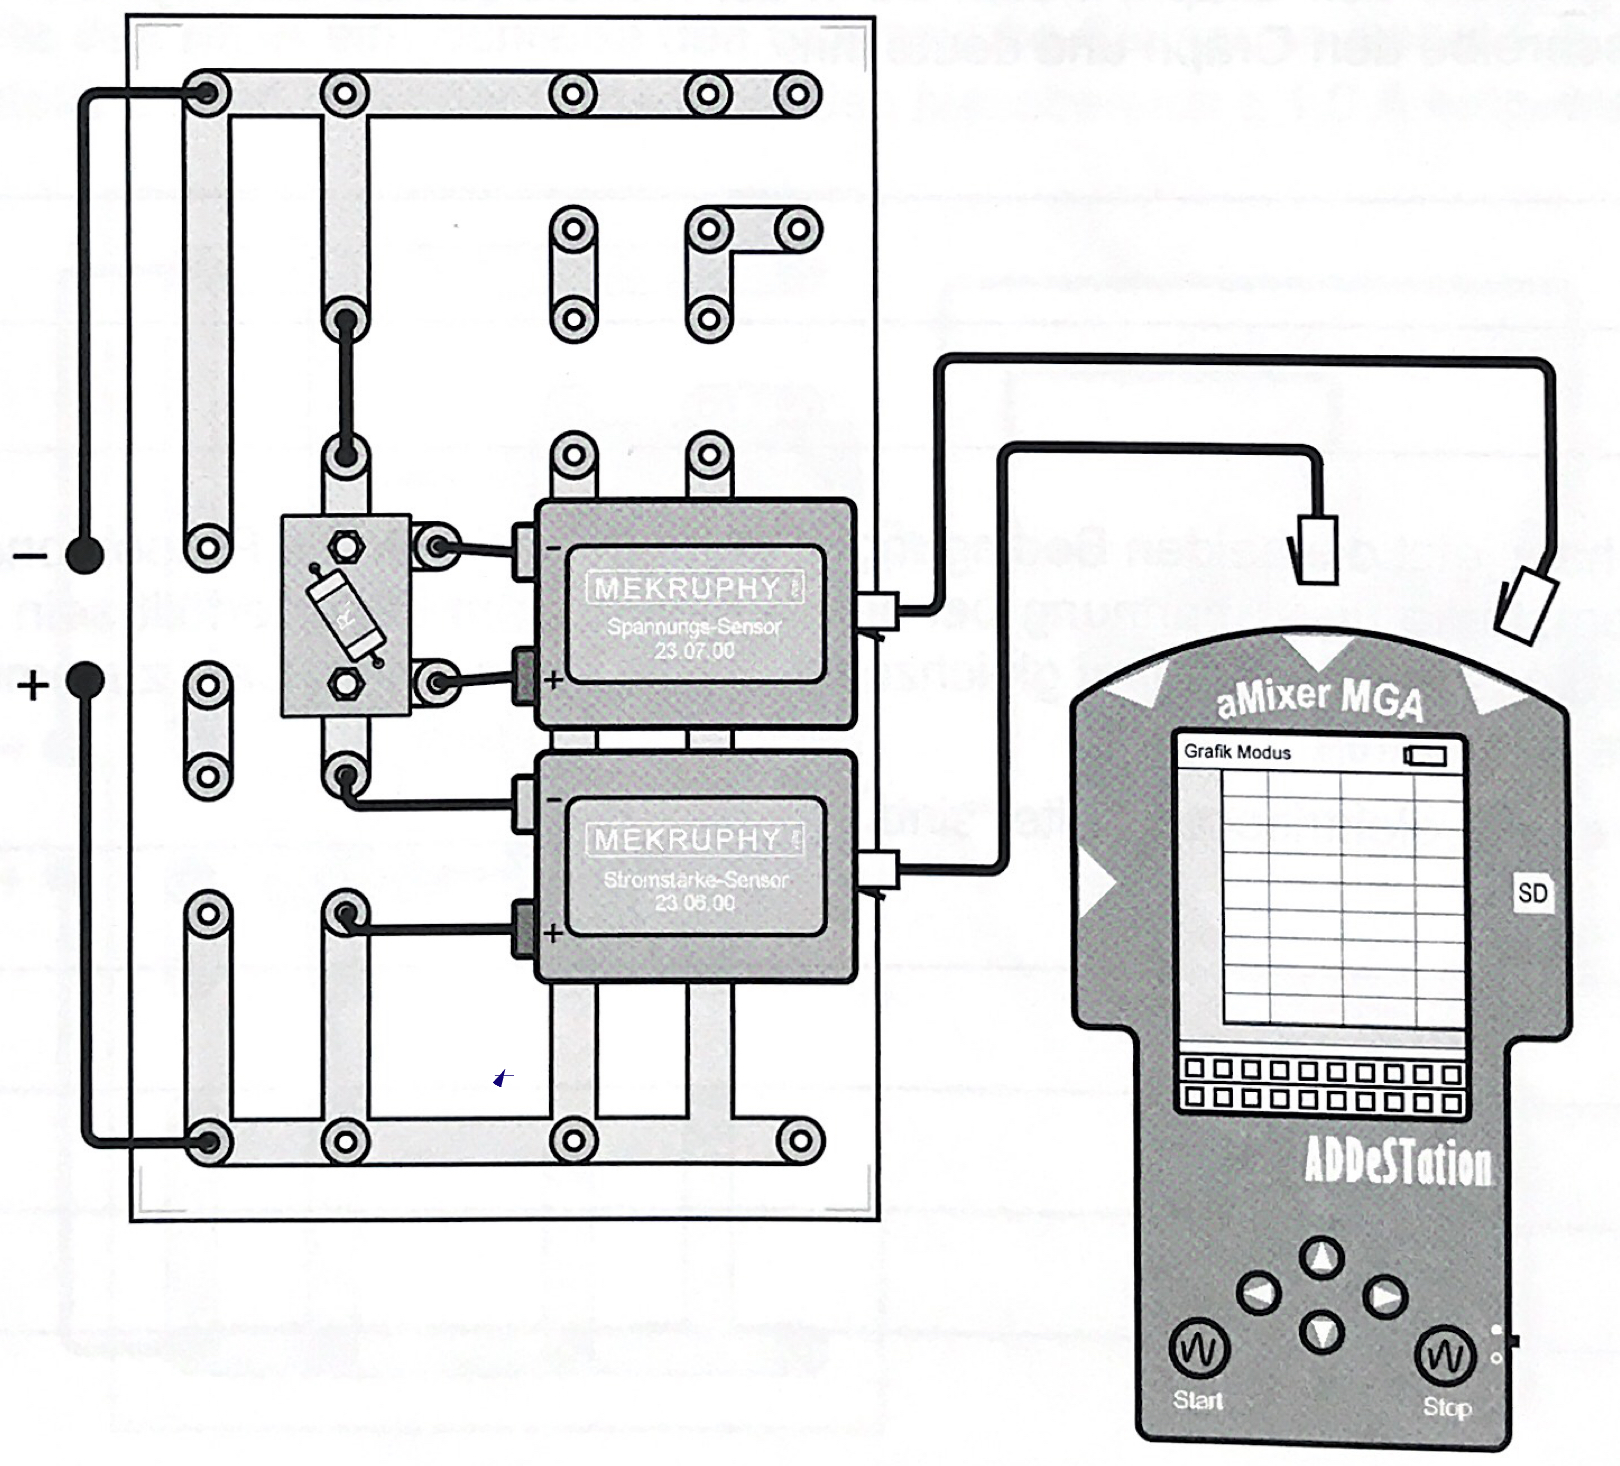
\includegraphics[width=.5\textwidth]{aufbau.jpg}
    \caption{Vorgegebener Versuchsaufbau (E5 - 3)}
    \label{fig:versuchsaufbau}
\end{figure}


%%%%%%%%    Beschreibung der Versuchsdurchführung   %%%%%%%%
\section{Beschreibung der Versuchsdurchführung}
Für den Versuch haben wir den Versuch aufgebaut wie vorgegeben in Abbildung \ref{fig:versuchsaufbau}, dann muss man das MGA richtig einstellen sowie konfigurieren.

In diesem Experiment geht es darum, Widerstandswerte zu bestimmen. Dazu wird das MGA eingeschaltet und der Spannungs-Sensor an Kanal 1 (CH 1) angeschlossen. Es ist wichtig, die Einstellung des Sensors auf den Messbereich von höchstens 6 V zu überprüfen. Der Stromstärke-Sensor wird ebenfalls angeschlossen, diesmal an Kanal 2 (CH 2) des MGA. Stellen Sie sicher, dass der Sensor auf den Messbereich von 1,0 A eingestellt ist. Die Sensoren müssen auf Nullstellung gebracht werden, und die Schaltung muss wie in der Abbildung \ref{fig:versuchsaufbau} aufgebaut werden. Allerdings sollte das Netzgerät noch nicht eingeschaltet werden. Der Drehknopf am Netzgerät muss auf Null stehen und die Polung muss richtig eingestellt sein.

Um die Messungen durchzuführen, müssen Sie in der Menüleiste auf das Symbol mit dem Schraubenschlüssel klicken. Es erscheint ein Fenster namens "EINSTELLUNGEN". Wenn "Input meine eigenen Daten" ausgewählt ist, tippen Sie auf "START". Andernfalls müssen Sie mit den Pfeiltasten die richtige Auswahl treffen. Tippen Sie auf das Feld "CH*" und bestätigen Sie die Kanäle durch Tippen auf das Feld "Fertig".

Schalten Sie das Netzgerät ein und tippen Sie auf das grün/rote Startfeld. Daraufhin erscheinen die aktuellen Spannungs- und Stromstärkewerte in der ersten Zeile. Regulieren Sie die Spannung auf etwa 1 V und tippen Sie erneut auf das grün/rote Startfeld. Daraufhin erscheinen in der zweiten Zeile die neuen Spannungs- und Stromstärkewerte. Wiederholen Sie diesen Prozess, indem Sie die Spannung in 1 V-Schritten bis etwa 5 V erhöhen. Regulieren Sie dann die Spannung auf null und schalten Sie das Netzgerät aus.

Um die Ergebnisse auszuwerten, tippen Sie in der Menüleiste auf das Symbol "G" und dann auf "Graph". Dadurch werden die Spannungswerte graphisch gegen die Stromstärkewerte aufgetragen. Diese liegen grob auf einer Geraden. Um diese Gerade zu erhalten, tippen Sie auf das Symbol "A". Daraufhin erscheint ein Fenster namens "Funktionsauswahl". Wählen Sie "lineare Regression" und tippen Sie dann auf "Fertig"\footnote{Unter idealen Bedingungen, da wir um weit mehrere Messungen gebraucht haben und die genausten gewählt haben haben wir die Regressionen auf einem TI-84 Taschenrechner gemacht.}. Die Steigung dieser Geraden ist ein Maß für den Widerstand. Sie erscheint in der angegebenen Gleichung y = a * x + b als Faktor a. 


%%%%%%%%    Messergebnisse mit Veranschaulichung   %%%%%%%%
\section{Messergebnisse und ggf. grafische Veranschaulichung}

%%%%%%%%%%% Tabelle R_1 %%%%%%%%%%%
\begin{table}[!htb]
\begin{minipage}[t]{.25\linewidth}
\centering
\caption{$R_1$}  
\label{tab:first_table}
 \resizebox{.7\linewidth}{!}{%
    \begin{tabular}{@{}ccc@{}}
    \toprule
    {U (V)} & {I (A)} & {R ($\Omega$)}\\
    \midrule
        1,05 & 0,15 & 7 \\
        2,01 & 0,30 & 6,7 \\
        3,14 & 0,46 & 6,83 \\
        4,12 & 0,62 & 6,65 \\
        4,86 & 0,73 & 6,66 \\
    \midrule
             &   Rø & 6,77 \\
    \bottomrule
    \end{tabular}%
}%
\end{minipage}%
\hfill%
%%%%%%%%%%% Tabelle R_2 %%%%%%%%%%%
\begin{minipage}[t]{.25\linewidth}
\centering
  \caption{$R_2$}
  \label{tab:second_table}
 \resizebox{.7\linewidth}{!}{%
 \begin{tabular}{@{}ccc@{}}
    \toprule
    {U (V)} & {I (A)} & {R ($\Omega$)}\\
    \midrule
        0,99 & 0,06 & 16,50\\
        2,00 & 0,13 & 15,38\\
        3,04 & 0,19 & 16,00\\
        4,05 & 0,25 & 16,20\\
        4,96 & 0,31 & 16,00\\
    \midrule
             &  Rø  & 16,02\\
    \bottomrule
    \end{tabular}%
  }%
\end{minipage}%
\hfill%
%%%%%%%%%%% Tabelle R_3 %%%%%%%%%%%
\begin{minipage}[t]{.25\linewidth}
\centering
 \caption{$R_3$} \label{tab:third_table}
 \resizebox{.7\linewidth}{!}{%
  \begin{tabular}{@{}ccc@{}}
    \toprule
    {U (V)} & {I (A)} & {R ($\Omega$)}\\
    \midrule
        1,01 & 0,04 & 25,25\\
        2,02 & 0,09 & 22,44\\
        3,01 & 0,13 & 23,15\\
        4,05 & 0,17 & 23,82\\
        5,06 & 0,22 & 23,00\\
    \midrule
             & Rø   & 23,53\\
    \bottomrule
    \end{tabular}%
 }%
\end{minipage}%
\hfill%
%%%%%%%%%%% Tabelle R_4 %%%%%%%%%%%
\begin{minipage}[t]{.25\linewidth}
\centering
  \caption{$R_4$}
  \label{tab:fourth_table}
 \resizebox{.7\linewidth}{!}{
 \begin{tabular}{@{}ccc@{}}
    \toprule
    {U (V)} & {I (A)} & {R ($\Omega$)}\\
    \midrule
        0,97 & 0,03 & 32,33\\
        1,96 & 0,05 & 39,20\\
        2,97 & 0,08 & 37,13\\
        4,06 & 0,10 & 40,60\\
        4,98 & 0,13 & 38,31\\
    \midrule
             &      & 37,51\\
    \bottomrule
    \end{tabular}%
}
\end{minipage} 
\end{table}


\textbf{Ergebnisse aus linearen Regressionen:}\\
$R_1$: $0,1520276096x - 0,009555823$    ($R^2$= 0,999601584)\\
$R_2$: $0,0620480938x + 0,0013593338$   ($R^2$= 0,999058159)\\
$R_3$: $0,0434312331x - 0,001596636$    ($R^2$= 0,997798999)\\
$R_4$: $0,0244937873x + 0,0248125637$   ($R^2$= 0,418763673).\\


\begin{center}
\definecolor{wvvxds}{rgb}{0.39,0.34,0.82}
\definecolor{dbwrru}{rgb}{0.85,0.38,0.07}
\definecolor{dtsfsf}{rgb}{0.82,0.18,0.18}
\definecolor{rvwvcq}{rgb}{0.082,0.39,0.75}

\begin{figure}[htb]
\centering
\begin{tikzpicture}[line cap=round,line join=round,>=triangle 45,x=2cm,y=10cm]
\begin{axis}[    x=2cm,    y=10cm,    axis lines=middle,    xmin=0,    xmax=5,    ymin=0,    ymax=0.3,    xtick={0,0.5,...,5},    ytick={0,0.1,...,0.7},    ]
%\clip(-0.09262467958279452,-0.028196653147060838) rectangle (2.7500061415409873,0.31595833620283137);
\draw[line width=2pt,color=rvwvcq,smooth,samples=100,domain=0:5] plot(\x,{0.1520276096*(\x)-0.009555823});
\draw[line width=2pt,color=dtsfsf,smooth,samples=100,domain=0:5] plot(\x,{0.0620480938*(\x)+0.0013593338});
\draw[line width=2pt,color=dbwrru,smooth,samples=100,domain=0:5] plot(\x,{0.0434312331*(\x)-0.001596636});
\draw[line width=2pt,color=wvvxds,smooth,samples=100,domain=0:5] plot(\x,{0.0244937873*(\x)+0.0248125637});
\begin{scriptsize}
\draw[color=rvwvcq] (0.25,0.25) node {$R_{1}$};
\draw[color=dtsfsf] (0.25,0.2) node {$R_{2}$};
\draw[color=dbwrru] (0.25,0.15) node {$R_{3}$};
\draw[color=wvvxds] (0.25,0.1) node {$R_{4}$};
\end{scriptsize}
\end{axis}
\end{tikzpicture}
\caption{Darstellung der Regressionen}
\label{fig:resistance}
\end{figure}
    
\end{center}

Das folgende Diagramm ist ohne die y-Achsen Verschiebungen, da diese nicht vorkommen sollten und aufgrund ungenauer Messungen und deren Regressionen entstanden, außerdem soll es der besseren Veranschaulichung helfen.

\begin{center}
\definecolor{wvvxds}{rgb}{0.39,0.34,0.82}
\definecolor{dbwrru}{rgb}{0.85,0.38,0.07}
\definecolor{dtsfsf}{rgb}{0.82,0.18,0.18}
\definecolor{rvwvcq}{rgb}{0.082,0.39,0.75}

\begin{figure}[htb]
\centering
\begin{tikzpicture}[line cap=round,line join=round,>=triangle 45,x=2cm,y=10cm]
\begin{axis}[    x=2cm,    y=10cm,    axis lines=middle,    xmin=0,    xmax=5,    ymin=0,    ymax=0.3,    xtick={0,0.5,...,5},    ytick={0,0.1,...,0.7},    ]
%\clip(-0.09262467958279452,-0.028196653147060838) rectangle (2.7500061415409873,0.31595833620283137);
\draw[line width=2pt,color=rvwvcq,smooth,samples=100,domain=0:5] plot(\x,{0.1520276096*(\x)});
\draw[line width=2pt,color=dtsfsf,smooth,samples=100,domain=0:5] plot(\x,{0.0620480938*(\x)});
\draw[line width=2pt,color=dbwrru,smooth,samples=100,domain=0:5] plot(\x,{0.0434312331*(\x)});
\draw[line width=2pt,color=wvvxds,smooth,samples=100,domain=0:5] plot(\x,{0.0244937873*(\x)});
\begin{scriptsize}
\draw[color=rvwvcq] (0.25,0.25) node {$R_{1}$};
\draw[color=dtsfsf] (0.25,0.2) node {$R_{2}$};
\draw[color=dbwrru] (0.25,0.15) node {$R_{3}$};
\draw[color=wvvxds] (0.25,0.1) node {$R_{4}$};
\end{scriptsize}
\end{axis}
\end{tikzpicture}
\caption{Gleiche Regressionen ohne y-achsen verschiebung}
\label{fig:resistance2}
\end{figure}    
\end{center}




%%%%%%%%%%% Fehlerbetrachtung %%%%%%%%%%%
\section{Fehlerbetrachtung}
Bei der Betrachtung des vorliegenden Problems wurden zwei systematische Hauptfehlerquellen identifiziert:
\begin{itemize}
    \item Das Netzteil ist sehr ungenau und gibt eine Spannung nur in einem Rahmen von ±3 Volt an, obwohl der erwartete Bereich 1-6 Volt beträgt.
    \item  Das verwendete Messgerät ist nicht sicher genau, was zu Messfehlern führen kann.
\end{itemize}
Um diese Fehlerquellen zu minimieren und genaue Messwerte zu erhalten, wurden mehrere hundert Messungen durchgeführt. Durch die Durchführung einer großen Anzahl von Messungen konnte eine Toleranz von 0,05 Volt erreicht werden.

Um zukünftige Messungen genauer zu gestalten, sollten geeignete Schritte zur Fehlerminimierung unternommen werden, wie beispielsweise die Verwendung von präziseren Messgeräten und die Kalibrierung des Netzteil auf den erwarteten Bereich. Dies kann die Messgenauigkeit verbessern und die Anzahl der erforderlichen Messungen reduzieren.

%%%%%%%%%%% Schlussfolgerung %%%%%%%%%%%
\section{Interpretation und Schlussfolgerung}

Zusammenfassend lässt sich sagen, dass die Ergebnisse des Versuchs das Ohm'sche Gesetz bestätigen. Die linearen Regressionen zeigen eine proportionale Beziehung zwischen Stromstärke und Spannung bei allen getesteten Widerständen. Die Werte für den Widerstand, die durch die Regressionen erhalten wurden. Allerdings sollte beachtet werden, dass die Messgenauigkeit aufgrund von ungenauen Messgeräten und des Netzteil begrenzt ist. Daher sollten in Zukunft geeignete Maßnahmen ergriffen werden, um die Fehlerquellen zu minimieren und genauere Ergebnisse zu erzielen.




\end{document}